\apendice{Especificación de Requisitos}

\section{Introducción}

En este apartado se van a detallar los requisitos globales del proyecto presentado, así como los diferentes casos de uso y requisitos funcionales implementados en la aplicación.

\section{Objetivos generales}

A continuación se muestran los objetivos generales del proyecto:

\begin{itemize}
	\item Investigar las bibliotecas de Tensorflow y los modelos Mobilenet e Inception para crear clasificadores de imágenes que sean capaces de ejecutarse en arquitecturas móviles.
	\item Investigar técnicas de uso de la Web Semántica para recopilar información de las diferentes especies de setas, de forma automática.
	\item Investigar técnicas de Web Scraping para extraer gran cantidad de información de una página Web.
	\item Implementar una aplicación Android que a partir de un clasificador de imágenes y la realización de preguntas al usuario, determine la especie de una seta. Esta aplicación mostrará información de cada especie y filtrará las preguntas de la clave dicotómica de acuerdo a las especies devueltas por el clasificador.
	\item Generar una aplicación Java que extraiga la información de las especies y las claves dicotómicas de forma automática.
	\item Internacionalizar la aplicación Android de manera que se pueda visualizar tanto en Inglés como en Español.
\end{itemize}

\section{Catalogo de requisitos}

En esta sección se van a detallar los diferentes requisitos funcionales implementados en las diferentes aplicaciones y herramientas.

\begin{itemize}
	\item \textbf{RF.1} Crear una herramienta que nos permita descargar información de las diferentes especies de setas.
	\begin{itemize}
	\item \textbf{RF.1.1} Se introducirá un listado de las especies deseadas y la aplicación devolverá la información extraída de la DBpedia.
	\item \textbf{RF.1.2} La información se podrá descargar tanto en 	español como en inglés.
	\end{itemize}
	
	\item \textbf{RF.2} Crear una herramienta que nos permita descargar las diferentes claves dicotómicas.
	\begin{itemize}
	\item \textbf{RF.2.1} La aplicación devolverá una clave dicotómica que discrimine entre géneros de setas.
	\item \textbf{RF.2.2} La aplicación devolverá claves dicotómicas que discriminen entre las especies de diferentes géneros de setas.
	\item \textbf{RF.2.3} Las claves se extraerán en español y se traducirán automáticamente al inglés.
	\item \textbf{RF.2.4} Las claves se serializarán en estructuras de datos java para incorporarlas a la aplicación Android.
	\end{itemize}
	
	\item \textbf{RF.3} Generar una aplicación para crear una base de datos SQlite para almacenar la información descargada y exportarla a la aplicación Android. Permitirá las siguientes acciones:
	\begin{itemize}
	\item \textbf{RF.3.1} Almacenar la descripción de la especie en Español.
	\item \textbf{RF.3.2} Almacenar la descripción de la especie en Inglés.
	\item \textbf{RF.3.3} Almacenar la comestibilidad de la especie en Español.
	\item \textbf{RF.3.4} Almacenar la comestibilidad de la especie en Inglés.
	\item \textbf{RF.3.5} Almacenar el género de la especie.
	\item \textbf{RF.3.6} Almacenar un enlace que redirija a la página web de la seta en Wikipedia.
	\end{itemize}
	
	\item \textbf{RF.4} Usar los algoritmos de Python proporcionados en los ejemplos de Tensorflow para entrenar los clasificadores de imágenes. \url{https://github.com/tensorflow/tensorflow/tree/master/tensorflow/examples/image_retraining}
	\begin{itemize}
	\item \textbf{RF.4.1} Elegir el modelo de Mobilenet o Inception.
	\item \textbf{RF.4.2} Incorporar las imágenes de las especies de setas sobre las que se quiere entrenar el clasificador.
	\item \textbf{RF.4.3} Determinar el porcentaje de imágenes que van a ser recortadas para crear nuevas.
	\item \textbf{RF.4.4} Determinar el porcentaje de imágenes que van a ser escaladas para crear nuevas.
	\item \textbf{RF.4.5} Determinar el porcentaje de imágenes que se va a rotar para crear nuevas.
	\item \textbf{RF.4.6} Determinar el porcentaje de imágenes sobre las que se va a modificar el brillo para crear nuevas.
	\item \textbf{RF.4.7} Elegir el número de pasos que va a realizar el clasificador para entrenar el modelo.
	\end{itemize}
	
	\item \textbf{RF.5} Generar una aplicación Android que permita la clasificación de la especie de una seta con las siguientes funcionaldades:
	\begin{itemize}
	\item \textbf{RF.5.1} El usuario podrá introducir una imagen de la seta desde la cámara del móvil para clasificar.
	\item \textbf{RF.5.2} El usuario podrá guardar la imagen capturada desde la cámara.
	\item \textbf{RF.5.3} El usuario podrá introducir una imagen de la seta desde la galería del móvil para clasificar.
	\item \textbf{RF.5.4} La aplicación mostrará las especies más probables clasificadas para la imagen introducida.
	\item \textbf{RF.5.5} Se mostrará información e imágenes de ejemplo para cada especie obtenida como resultado.
	\item \textbf{RF.5.6} El usuario podrá comparar su imagen con las proporcionadas por la aplicación 
	\item \textbf{RF.5.7} La aplicación realizará preguntas al usuario para clasificar la especie y reforzar la tarea de clasificación.
	\item \textbf{RF.5.8} Se podrán filtrar las preguntas realizadas para que solo se realicen sobre las especies deseadas.
	\item \textbf{RF.5.9} El usuario podrá cambiar el idioma de la aplicación entre español e inglés.
	\item \textbf{RF.5.10} El usuario podrá acceder a la información de todas las especies a través de un listado de estas.
	\item \textbf{RF.5.11} El usuario podrá acceder a las claves dicotómicas de las especies a través de un listado de estas.
	\item \textbf{RF.5.12} La aplicación mostrará páginas de ayuda que guíen al usuario dentro de la aplicación.
	
	\end{itemize}
	
\end{itemize}


\section{Especificación de requisitos}

\subsection{Diagramas de casos de uso}

\begin{figure}[]
    \begin{center}%
        \begin{center}%
          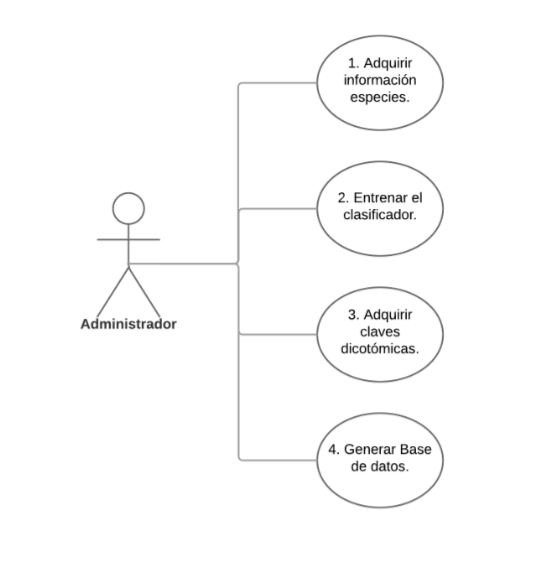
\includegraphics[width=1\textwidth]{imagenesAnexos/imagenesRequisitos/CasosDeUsoAdmin}%
          \caption{Diagrama de casos de uso del administrador.}%
          \label{figCasosUsoAdmin}%
        \end{center}%
  	\end{center}%
\end{figure}%

\begin{figure}[]
    \begin{center}%
        \begin{center}%
          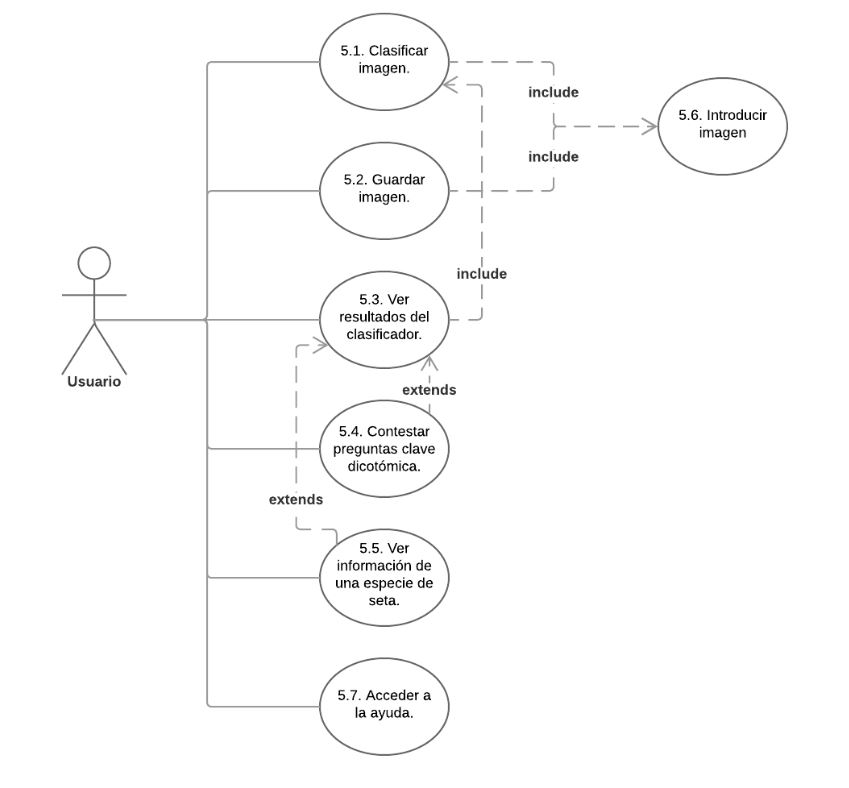
\includegraphics[width=1\textwidth]{imagenesAnexos/imagenesRequisitos/CasosDeUsoUser}%
          \caption{Diagrama de casos de uso del usuario.}%
          \label{figCasosUsoUser}%
        \end{center}%
  	\end{center}%
\end{figure}%
 
\newpage

\subsection{Especificación de los casos de uso}


%CASO DE USO 1

\tablaSmallSinColores{Caso de uso 1: Adquirir información especies.}{p{3cm} p{.75cm} p{9.5cm}}{tablaUC1}{
  \multicolumn{3}{l}{Caso de uso 1:  Adquirir información especies.} \\
 }
 {
  Descripción                            & \multicolumn{2}{p{10.25cm}}{Permite al administrador extraer la información de la especies de la DBpedia.} \\\hline
  \multirow{2}{3.5cm}{Requisitos}   &\multicolumn{2}{p{10.25cm}}{RF-1} \\\cline{2-3}
                                         & \multicolumn{2}{p{10.25cm}}{RF-1.1} \\\cline{2-3}
                                         & \multicolumn{2}{p{10.25cm}}{RF-1.2} 
                                         \\\hline
  Precondiciones                         &  \multicolumn{2}{p{10.25cm}}{Se necesita conexión a Internet para acceder a la DBpedia y tener creadas las tablas en la base de datos SQlite.}   \\\hline
  \multirow{2}{3.5cm}{Secuencia normal}  & Paso & Acción \\\cline{2-3}
                                         & 1    & El administrador indica la ruta de la base de datos.
  \\\cline{2-3}
                                         & 2    & Se inserta un listado de las especies a descargar.
  \\\cline{2-3}
                                         & 3    & Se inicia el programa
    \\\cline{2-3}
                                         & 4    & Se carga la base de datos con la información extraída de la DBpedia. 
                                         \\\hline
  Postcondiciones                        & \multicolumn{2}{p{10.25cm}}{Se ha descargado la información de la especies de setas.} \\\hline
  Excepciones                        & \multicolumn{2}{p{10.25cm}}{No se ha podido acceder a la DBpedia.}\\\hline
  Importancia                            & Media \\\hline
  Urgencia                               & Media \\
}

%CASO DE USO 2

\tablaSmallSinColores{Caso de uso 2: Entrenar el clasificador.}{p{3cm} p{.75cm} p{9.5cm}}{tablaUC2}{
  \multicolumn{3}{l}{Caso de uso 2: Entrenar el clasificador.} \\
 }
 {
  Descripción                            & \multicolumn{2}{p{10.25cm}}{Permite al administrador reentrenar el clasificador de imágenes.} \\\hline
  \multirow{2}{3.5cm}{Requisitos}   &\multicolumn{2}{p{10.25cm}}{RF-4} \\\cline{2-3}
                                         & \multicolumn{2}{p{10.25cm}}{RF-4.1} \\\cline{2-3}
                                         & \multicolumn{2}{p{10.25cm}}{RF-4.2} \\\cline{2-3}
                                         & \multicolumn{2}{p{10.25cm}}{RF-4.3} \\\cline{2-3}
                                         & \multicolumn{2}{p{10.25cm}}{RF-4.4} \\\cline{2-3}
                                         & \multicolumn{2}{p{10.25cm}}{RF-4.5} \\\cline{2-3}
                                         & \multicolumn{2}{p{10.25cm}}{RF-4.6} \\\cline{2-3}
                                         & \multicolumn{2}{p{10.25cm}}{RF-4.7}
                                         \\\hline
  Precondiciones                         &  \multicolumn{2}{p{10.25cm}}{Tener instalado Tensorflow y Python en el sistema.}   \\\hline
  \multirow{2}{3.5cm}{Secuencia normal}  & Paso & Acción \\\cline{2-3}
                                         & 1    & Se indica el modelo a reentrenar.
  \\\cline{2-3}
                                         & 2    & Se incorporan las imágenes con las que se quiere entrenar.
  \\\cline{2-3}
                                         & 3    & Se ajustan los parámetros para realizar el Data Augmentation.
  \\\cline{2-3}
                                         & 4    & Se elige el número de pasos que va a realizar el programa para entrenar
  \\\cline{2-3}
                                         & 5    & Se inicia el programa.

                                         \\\hline
  Postcondiciones                        & \multicolumn{2}{p{10.25cm}}{Se ha entrenado un modelo para clasificar especies de setas.} \\\hline
  Excepciones                        & \multicolumn{2}{p{10.25cm}}{Número insuficiente de imágenes para entrenar.}\\\hline
  Importancia                            & Alta \\\hline
  Urgencia                               & Alta \\
}

%CASO DE USO 3

\tablaSmallSinColores{Caso de uso 3: Adquirir claves dicotómicas.}{p{3cm} p{.75cm} p{9.5cm}}{tablaUC3}{
  \multicolumn{3}{l}{Caso de uso 3: Adquirir claves dicotómicas.} \\
 }
 {
  Descripción                            & \multicolumn{2}{p{10.25cm}}{Permite al administrador extraer las claves de la página Web \url{http://www.avelinosetas.info/claves.php}.} \\\hline
  \multirow{2}{3.5cm}{Requisitos}   &\multicolumn{2}{p{10.25cm}}{RF-2} \\\cline{2-3}
                                         & \multicolumn{2}{p{10.25cm}}{RF-2.1} \\\cline{2-3}
                                         & \multicolumn{2}{p{10.25cm}}{RF-2.2} \\\cline{2-3}
                                         & \multicolumn{2}{p{10.25cm}}{RF-2.3} \\\cline{2-3}
                                         & \multicolumn{2}{p{10.25cm}}{RF-2.4} 
                                         \\\hline
  Precondiciones                         &  \multicolumn{2}{p{10.25cm}}{Se necesita conexión a Internet para acceder a la página web.}   \\\hline
  \multirow{2}{3.5cm}{Secuencia normal}  & Paso & Acción \\\cline{2-3}
                                         & 1    & El administrador indica el nombre del archivo donde se quiere exportar las claves.
  \\\cline{2-3}
                                         & 2    & Se inserta un listado de las claves a descargar.
  \\\cline{2-3}
                                         & 3    & Se inicia el programa
    \\\cline{2-3}
                                         & 4    & Se descargan las claves y se serializan en el archivo indicado.
                                         \\\hline
  Postcondiciones                        & \multicolumn{2}{p{10.25cm}}{Se obtienen las claves en un archivo serializado para ser exportado a la aplicación Android.} \\\hline
  Excepciones                        & \multicolumn{2}{p{10.25cm}}{No se ha podido acceder a la página web.}\\\hline
  Importancia                            & Alta \\\hline
  Urgencia                               & Media \\
}

%CASO DE USO 4

\tablaSmallSinColores{Caso de uso 4: Generar Base de datos.}{p{3cm} p{.75cm} p{9.5cm}}{tablaUC4}{
  \multicolumn{3}{l}{Caso de uso 4: Generar Base de datos.} \\
 }
 {
  Descripción                            & \multicolumn{2}{p{10.25cm}}{Permite al administrador preparar la base de datos para almacenar la información de las setas.} \\\hline
  \multirow{2}{3.5cm}{Requisitos}   &\multicolumn{2}{p{10.25cm}}{RF-1} \\\cline{2-3}
                                         & \multicolumn{2}{p{10.25cm}}{RF-2}
                                         \\\hline
  Precondiciones                         &  \multicolumn{2}{p{10.25cm}}{Haber creado una base de datos SQlite en el sistema.}   \\\hline
  \multirow{2}{3.5cm}{Secuencia normal}  & Paso & Acción \\\cline{2-3}
                                         & 1    & El administrador indica la ruta donde se encuentra la base de datos SQlite.
  \\\cline{2-3}
                                         & 2    & Se inicia el programa.
  \\\cline{2-3}
                                         & 3    & El programa crea las tablas necesarias en la base de datos.
                                         \\\hline
  Postcondiciones                        & \multicolumn{2}{p{10.25cm}}{Se crean las tablas en la base de datos.} \\\hline
  Excepciones                        & \multicolumn{2}{p{10.25cm}}{Excepción SQL.}\\\hline
  Importancia                            & Media \\\hline
  Urgencia                               & Media \\
}

%CASO DE USO 5

\tablaSmallSinColores{Caso de uso 5.1: Clasificar imagen.}{p{3cm} p{.75cm} p{9.5cm}}{tablaUC5}{
  \multicolumn{3}{l}{Caso de uso 5.1: Clasificar imagen.} \\
 }
 {
  Descripción                            & \multicolumn{2}{p{10.25cm}}{Permite al usuario clasificar la especie a la que pertenece la seta que aparezca en la foto introducida.} \\\hline
  \multirow{2}{3.5cm}{Requisitos}   &\multicolumn{2}{p{10.25cm}}{RF-5} \\\cline{2-3}
                                         & \multicolumn{2}{p{10.25cm}}{RF-5.4}
                                         \\\hline
  Precondiciones                         &  \multicolumn{2}{p{10.25cm}}{Haber cargado la imagen a clasificar.}   \\\hline
  \multirow{2}{3.5cm}{Secuencia normal}  & Paso & Acción \\\cline{2-3}
                                         & 1    & El usuario pulsa en el botón de clasificar, bien desde la actividad lanzadora o desde el menú.
  \\\cline{2-3}
                                         & 2    & El usuario carga la imagen deseada.
  \\\cline{2-3}
                                         & 3    & El usuario pulsa sobre el botón de clasificar la imagen.
  \\\cline{2-3}
                                         & 4    & El sistema muestra las especies más probables clasificadas para esa imagen.
                                         \\\hline
  Postcondiciones                        & \multicolumn{2}{p{10.25cm}}{Se muestran los resultados obtenidos.} \\\hline
  Excepciones                        & \multicolumn{2}{p{10.25cm}}{Error en la carga de la imágen. Error en la clasificación.}\\\hline
  Importancia                            & Alta \\\hline
  Urgencia                               & Alta \\
}

%CASO DE USO 6

\tablaSmallSinColores{Caso de uso 5.2: Guardar imagen.}{p{3cm} p{.75cm} p{9.5cm}}{tablaUC6}{
  \multicolumn{3}{l}{Caso de uso 5.2: Guardar imagen.} \\
 }
 {
  Descripción                            & \multicolumn{2}{p{10.25cm}}{Permite al usuario guardar en el sistema la imagen que haya capturado desde el móvil.} \\\hline
  \multirow{2}{3.5cm}{Requisitos}   &\multicolumn{2}{p{10.25cm}}{RF-5} \\\cline{2-3}
                                         & \multicolumn{2}{p{10.25cm}}{RF-5.2}
                                         \\\hline
  Precondiciones                         &  \multicolumn{2}{p{10.25cm}}{Tener acceso a la cámara del móvil.}   \\\hline
  \multirow{2}{3.5cm}{Secuencia normal}  & Paso & Acción \\\cline{2-3}
                                         & 1    & El usuario pulsa en el botón de clasificar, bien desde la actividad lanzadora o desde el menú.
  \\\cline{2-3}
                                         & 2    & El usuario elije la opción de cargar la imagen desde el móvil.
  \\\cline{2-3}
                                         & 3    & Se introduce la imagen.
  \\\cline{2-3}
                                         & 4    & El usuario pulsa sobre el botón de guardar.
                                         \\\hline
  Postcondiciones                        & \multicolumn{2}{p{10.25cm}}{Se almacena la imagen en la galería del móvil.} \\\hline
  Excepciones                        & \multicolumn{2}{p{10.25cm}}{Error en la carga de la imágen. Error al adquirir los permisos del móvil.}\\\hline
  Importancia                            & Baja \\\hline
  Urgencia                               & Baja \\
}

%CASO DE USO 7

\tablaSmallSinColores{Caso de uso 5.3: Ver resultados del clasificador.}{p{3cm} p{.75cm} p{9.5cm}}{tablaUC7}{
  \multicolumn{3}{l}{Caso de uso 5.3: Ver resultados del clasificador.} \\
 }
 {
  Descripción                            & \multicolumn{2}{p{10.25cm}}{Permite al usuario ver los resultados obtenidos de la clasificación y obtener información de las especies.} \\\hline
  \multirow{2}{3.5cm}{Requisitos}   &\multicolumn{2}{p{10.25cm}}{RF-5} \\\cline{2-3}
                                         & \multicolumn{2}{p{10.25cm}}{RF-5.4}
                                         \\\cline{2-3}
                                         & \multicolumn{2}{p{10.25cm}}{RF-5.5}
                                         \\\cline{2-3}
                                         & \multicolumn{2}{p{10.25cm}}{RF-5.6}
                                         \\\hline
  Precondiciones                         &  \multicolumn{2}{p{10.25cm}}{}   \\\hline
  \multirow{2}{3.5cm}{Secuencia normal}  & Paso & Acción \\\cline{2-3}
                                         & 1    & El usuario ha clasificado una imagen.
  \\\cline{2-3}
                                         & 2    & El sistema muestra una lista con los resultados obtenidos.
  \\\cline{2-3}
                                         & 3    & Si el usuario pulsa una especie de los resultados, se mostrará una imagen de ejemplo que se comparará con la introducida por el usuario.
  \\\cline{2-3}
                                         & 4    & Si el usuario mantiene pulsada una especie de los resultados, se mostrará información describiendo la especie.
                                         \\\hline
  Postcondiciones                        & \multicolumn{2}{p{10.25cm}}{Se muestra información de los resultados} \\\hline
  Excepciones                        & \multicolumn{2}{p{10.25cm}}{Error en la carga de la imágen. Error al acceder a la base de datos.}\\\hline
  Importancia                            & Media \\\hline
  Urgencia                               & Media \\
}

%CASO DE USO 8

\tablaSmallSinColores{Caso de uso 5.4: Contestar preguntas clave dicotómica.}{p{3cm} p{.75cm} p{9.5cm}}{tablaUC8}{
  \multicolumn{3}{l}{Caso de uso 5.4: Contestar preguntas clave dicotómica.} \\
 }
 {
  Descripción                            & \multicolumn{2}{p{10.25cm}}{El sistema realiza una serie de preguntas al usuario con el fin de clasificar el género o especie de la seta.} \\\hline
  \multirow{2}{3.5cm}{Requisitos}   &\multicolumn{2}{p{10.25cm}}{RF-5} \\\cline{2-3}
                                         & \multicolumn{2}{p{10.25cm}}{RF-5.7}
                                         \\\cline{2-3}
                                         & \multicolumn{2}{p{10.25cm}}{RF-5.8}
                                         \\\hline
  Precondiciones                         &  \multicolumn{2}{p{10.25cm}}{}   \\\hline
  \multirow{2}{3.5cm}{Secuencia después de clasificar una imagen.}  & Paso & Acción \\\cline{2-3}
                                         & 1    & El usuario clasifica una imagen.
  \\\cline{2-3}
                                         & 2    & Se pulsa el botón de acceder a la clave dicotómica.
  \\\cline{2-3}
                                         & 3    & El usuario puede elegir sobre que especies filtrar las preguntas o realizar todas las preguntas.
  \\\cline{2-3}
                                         & 4    & Una vez seleccionadas las especies, se pulsa sobre el botón de clasificar.
  \\\cline{2-3}
                                         & 5    & El usuario va respondiendo a las preguntas que le aparecen hasta que se muestra la especie clasificada.
                                         \\\hline
                                         \multirow{2}{3.5cm}{Secuencia desde el listado de claves}  & Paso & Acción \\\cline{2-3}
                                         & 1    & El usuario pulsa el botón de mostrar claves.
  \\\cline{2-3}
                                         & 2    & El sistema muestra una lista con las claves disponibles.
  \\\cline{2-3}
                                         & 3    & El usuario elije una clave.
  \\\cline{2-3}
                                         & 4    & El usuario va respondiendo a las preguntas que le aparecen hasta que se muestra la especie clasificada.
                                         \\\hline
  Postcondiciones                        & \multicolumn{2}{p{10.25cm}}{Se clasifica la especie de la seta mediante una clave dicotómica.} \\\hline
  Excepciones                        & \multicolumn{2}{p{10.25cm}}{}\\\hline
  Importancia                            & Alta \\\hline
  Urgencia                               & Alta \\
}

%CASO DE USO 9

\tablaSmallSinColores{Caso de uso 5.5: Ver información de una especie de seta.}{p{3cm} p{.75cm} p{9.5cm}}{tablaUC9}{
  \multicolumn{3}{l}{Caso de uso 5.5: Ver información de una especie de seta.} \\
 }
 {
  Descripción                            & \multicolumn{2}{p{10.25cm}}{El sistema muestra información de una especie de seta.} \\\hline
  \multirow{2}{3.5cm}{Requisitos}   &\multicolumn{2}{p{10.25cm}}{RF-5} \\\cline{2-3}
                                         & \multicolumn{2}{p{10.25cm}}{RF-5.10}
                                         \\\cline{2-3}
                                         & \multicolumn{2}{p{10.25cm}}{RF-5.5}
                                         \\\hline
  Precondiciones                         &  \multicolumn{2}{p{10.25cm}}{}   \\\hline
  \multirow{2}{3.5cm}{Secuencia desde los resultados.}  & Paso & Acción \\\cline{2-3}
                                         & 1    & El usuario clasifica una imagen.
  \\\cline{2-3}
                                         & 2    & Se mantiene pulsado sobre uno de los resultados.
  \\\cline{2-3}
                                         & 3    & El sistema muestra información de la especie seleccionada.
                                         \\\hline
                                         \multirow{2}{3.5cm}{Secuencia desde el listado de especies.}  & Paso & Acción \\\cline{2-3}
                                         & 1    & El usuario pulsa el botón de mostrar setas.
  \\\cline{2-3}
                                         & 2    & El sistema muestra una lista con las especies de setas disponibles.
  \\\cline{2-3}
                                         & 3    & El usuario elije una especie.
  \\\cline{2-3}
                                         & 4    & El sistema muestra información de la especie seleccionada.
                                         \\\hline
  Postcondiciones                        & \multicolumn{2}{p{10.25cm}}{Se muestra información de la especie seleccionada.} \\\hline
  Excepciones                        & \multicolumn{2}{p{10.25cm}}{}\\\hline
  Importancia                            & Media \\\hline
  Urgencia                               & Media \\
}

%CASO DE USO 10

\tablaSmallSinColores{Caso de uso 5.6: Introducir imagen.}{p{3cm} p{.75cm} p{9.5cm}}{tablaUC10}{
  \multicolumn{3}{l}{Caso de uso 5.6: Introducir imagen.} \\
 }
 {
  Descripción                            & \multicolumn{2}{p{10.25cm}}{El sistema permite al usuario introducir una imagen desde la cámara del móvil o desde la galería.} \\\hline
  \multirow{2}{3.5cm}{Requisitos}   &\multicolumn{2}{p{10.25cm}}{RF-5} \\\cline{2-3}
                                         & \multicolumn{2}{p{10.25cm}}{RF-5.1}
                                         \\\cline{2-3}
                                         & \multicolumn{2}{p{10.25cm}}{RF-5.3}
                                         \\\hline
  Precondiciones                         &  \multicolumn{2}{p{10.25cm}}{}   \\\hline
  \multirow{2}{3.5cm}{Secuencia desde la cámara}  & Paso & Acción \\\cline{2-3}
                                         & 1    & El usuario pulsa sobre el botón de clasificar.
  \\\cline{2-3}
                                         & 2    & El usuario selecciona el botón de la cámara.
  \\\cline{2-3}
                                         & 3    & Se captura la imagen.
                                         \\\hline
                                         \multirow{2}{3.5cm}{Secuencia desde la galería}  & Paso & Acción \\\cline{2-3}
                                         & 1    & El usuario pulsa sobre el botón de clasificar.
  \\\cline{2-3}
                                         & 2    & El usuario selecciona el botón de la galería.
  \\\cline{2-3}
                                         & 3    & Se selecciona la imagen de la galería.
                                         \\\hline
  Postcondiciones                        & \multicolumn{2}{p{10.25cm}}{El sistema carga la imagen para ser clasificada.} \\\hline
  Excepciones                        & \multicolumn{2}{p{10.25cm}}{}\\\hline
  Importancia                            & Alta \\\hline
  Urgencia                               & Alta \\
}

%CASO DE USO 11

\tablaSmallSinColores{Caso de uso 5.7: Acceder a la ayuda.}{p{3cm} p{.75cm} p{9.5cm}}{tablaUC11}{
  \multicolumn{3}{l}{Caso de uso 5.7: Acceder a la ayuda.} \\
 }
 {
  Descripción                            & \multicolumn{2}{p{10.25cm}}{El sistema permite al usuario acceder a la ayuda de cada actividad desde el menú o desde el botón de ayuda.} \\\hline
  \multirow{2}{3.5cm}{Requisitos}   &\multicolumn{2}{p{10.25cm}}{RF-5} \\\cline{2-3}
                                         & \multicolumn{2}{p{10.25cm}}{RF-5.12}
                                         \\\hline
  Precondiciones                         &  \multicolumn{2}{p{10.25cm}}{}   \\\hline
  \multirow{2}{3.5cm}{Secuencia normal}  & Paso & Acción \\\cline{2-3}
                                         & 1    & El usuario pulsa sobre el botón de ayuda del menú o de la actividad actual.
  \\\cline{2-3}
                                         & 2    & El sistema muestra la ayuda de la actividad o del menú.
                                         \\\hline
                                        
  Postcondiciones                        & \multicolumn{2}{p{10.25cm}}{El sistema muestra la ayuda.} \\\hline
  Excepciones                        & \multicolumn{2}{p{10.25cm}}{}\\\hline
  Importancia                            & Media \\\hline
  Urgencia                               & Media \\
}
